%!TEX root = ../SciVis.tex

%The aim of this step is for you to understand and implement a set of vector field operators. Vector field operators are used to compute various quantities on vector fields, which enable different types of analyses to take place on the vector data. In this step, you will implement the computation of the divergence operator. Informally put: the divergence of a vector field v, denoted as div v, is a scalar quantity which shows, at every point, the amount of mass which is compressed or expanded when it would be flowing in that field. A divergence value of zero means the field neither compresses nor expands (dilates) mass as it carries it along (advects it). If mass enters the field at some point, called a source point, then that point will have a positive divergence value. If mass exits the field at some point, called a sink point, then that point will have a negative divergence value.
% 
%In this step, you have to implement the following:
% 
%�        Compute the divergence div v of the fluid velocity field v. This will deliver a scalar field, sampled on the same grid as the velocity field. Next, add an option to visualize the divergence field, using the color mapping functionality implemented in step 2.
%�        Do the same as above, now for the force field f. What relation do you see between the divergence div f and the force field magnitude | f | itself?
% 
%Hints: Start from the divergence definition. Compute the partial derivatives in this definition directly from the discrete data available on the simulation�s grid. For this, see Chapter 3 � Section 3.7.

In this step the implementation and analysis of the divergence operator will be introduced. Divergence is a vector field operator and as such it is applied either to the velocity vector dataset or the force vector dataset. The user can select from which vector dataset the divergence will be computed ---\emph{Div Velocity} or \emph{Div Force}--- from the \emph{Scalar} listbox which can be found in the \emph{Dataset} panel. The divergence operator is computed with the following code depicted in Listing~\ref{lst:divergence}.

\begin{lstlisting}[language=C,label=lst:divergence,caption={Divergence of the velocity vector dataset.}]
float Visualization::divergence(Simulation const &simulation, int idx) {
	int DIM = Simulation::DIM;
	int x = idx % DIM;
	int y = idx / DIM;
	int right = modIndex(x + 1, y, DIM);
	int left = modIndex(x - 1, y, DIM);
	int top = modIndex(x, y - 1, DIM);
	int bottom = modIndex(x, y + 1, DIM);

	float dx = 0.0;
	float dy = 0.0;

	dx = simulation.vx[right] - simulation.vx[left];
	dy = simulation.vy[top] - simulation.vy[bottom];

	return dx + dy;
}
 \end{lstlisting}

Figure~\ref{fig:divergenceVelocity} depicts the divergence of the \emph{Velocity} vector dataset regularly sampled at 80x80 and coloured with a heatmap colormap. The range that the values are clamped is selected to be -0.01 to 0.03. This because divergence can have negative values. The black colors on Figure~\ref{fig:divergenceVelocity} denotes sink points, negative values, while the yellow and white colors denote sources, positive values. At these source points it is where the force is applied. At these points the smoke starts spreading and this is the reason that the divergence has positive values.

\begin{figure}[htbp]
\begin{center}
 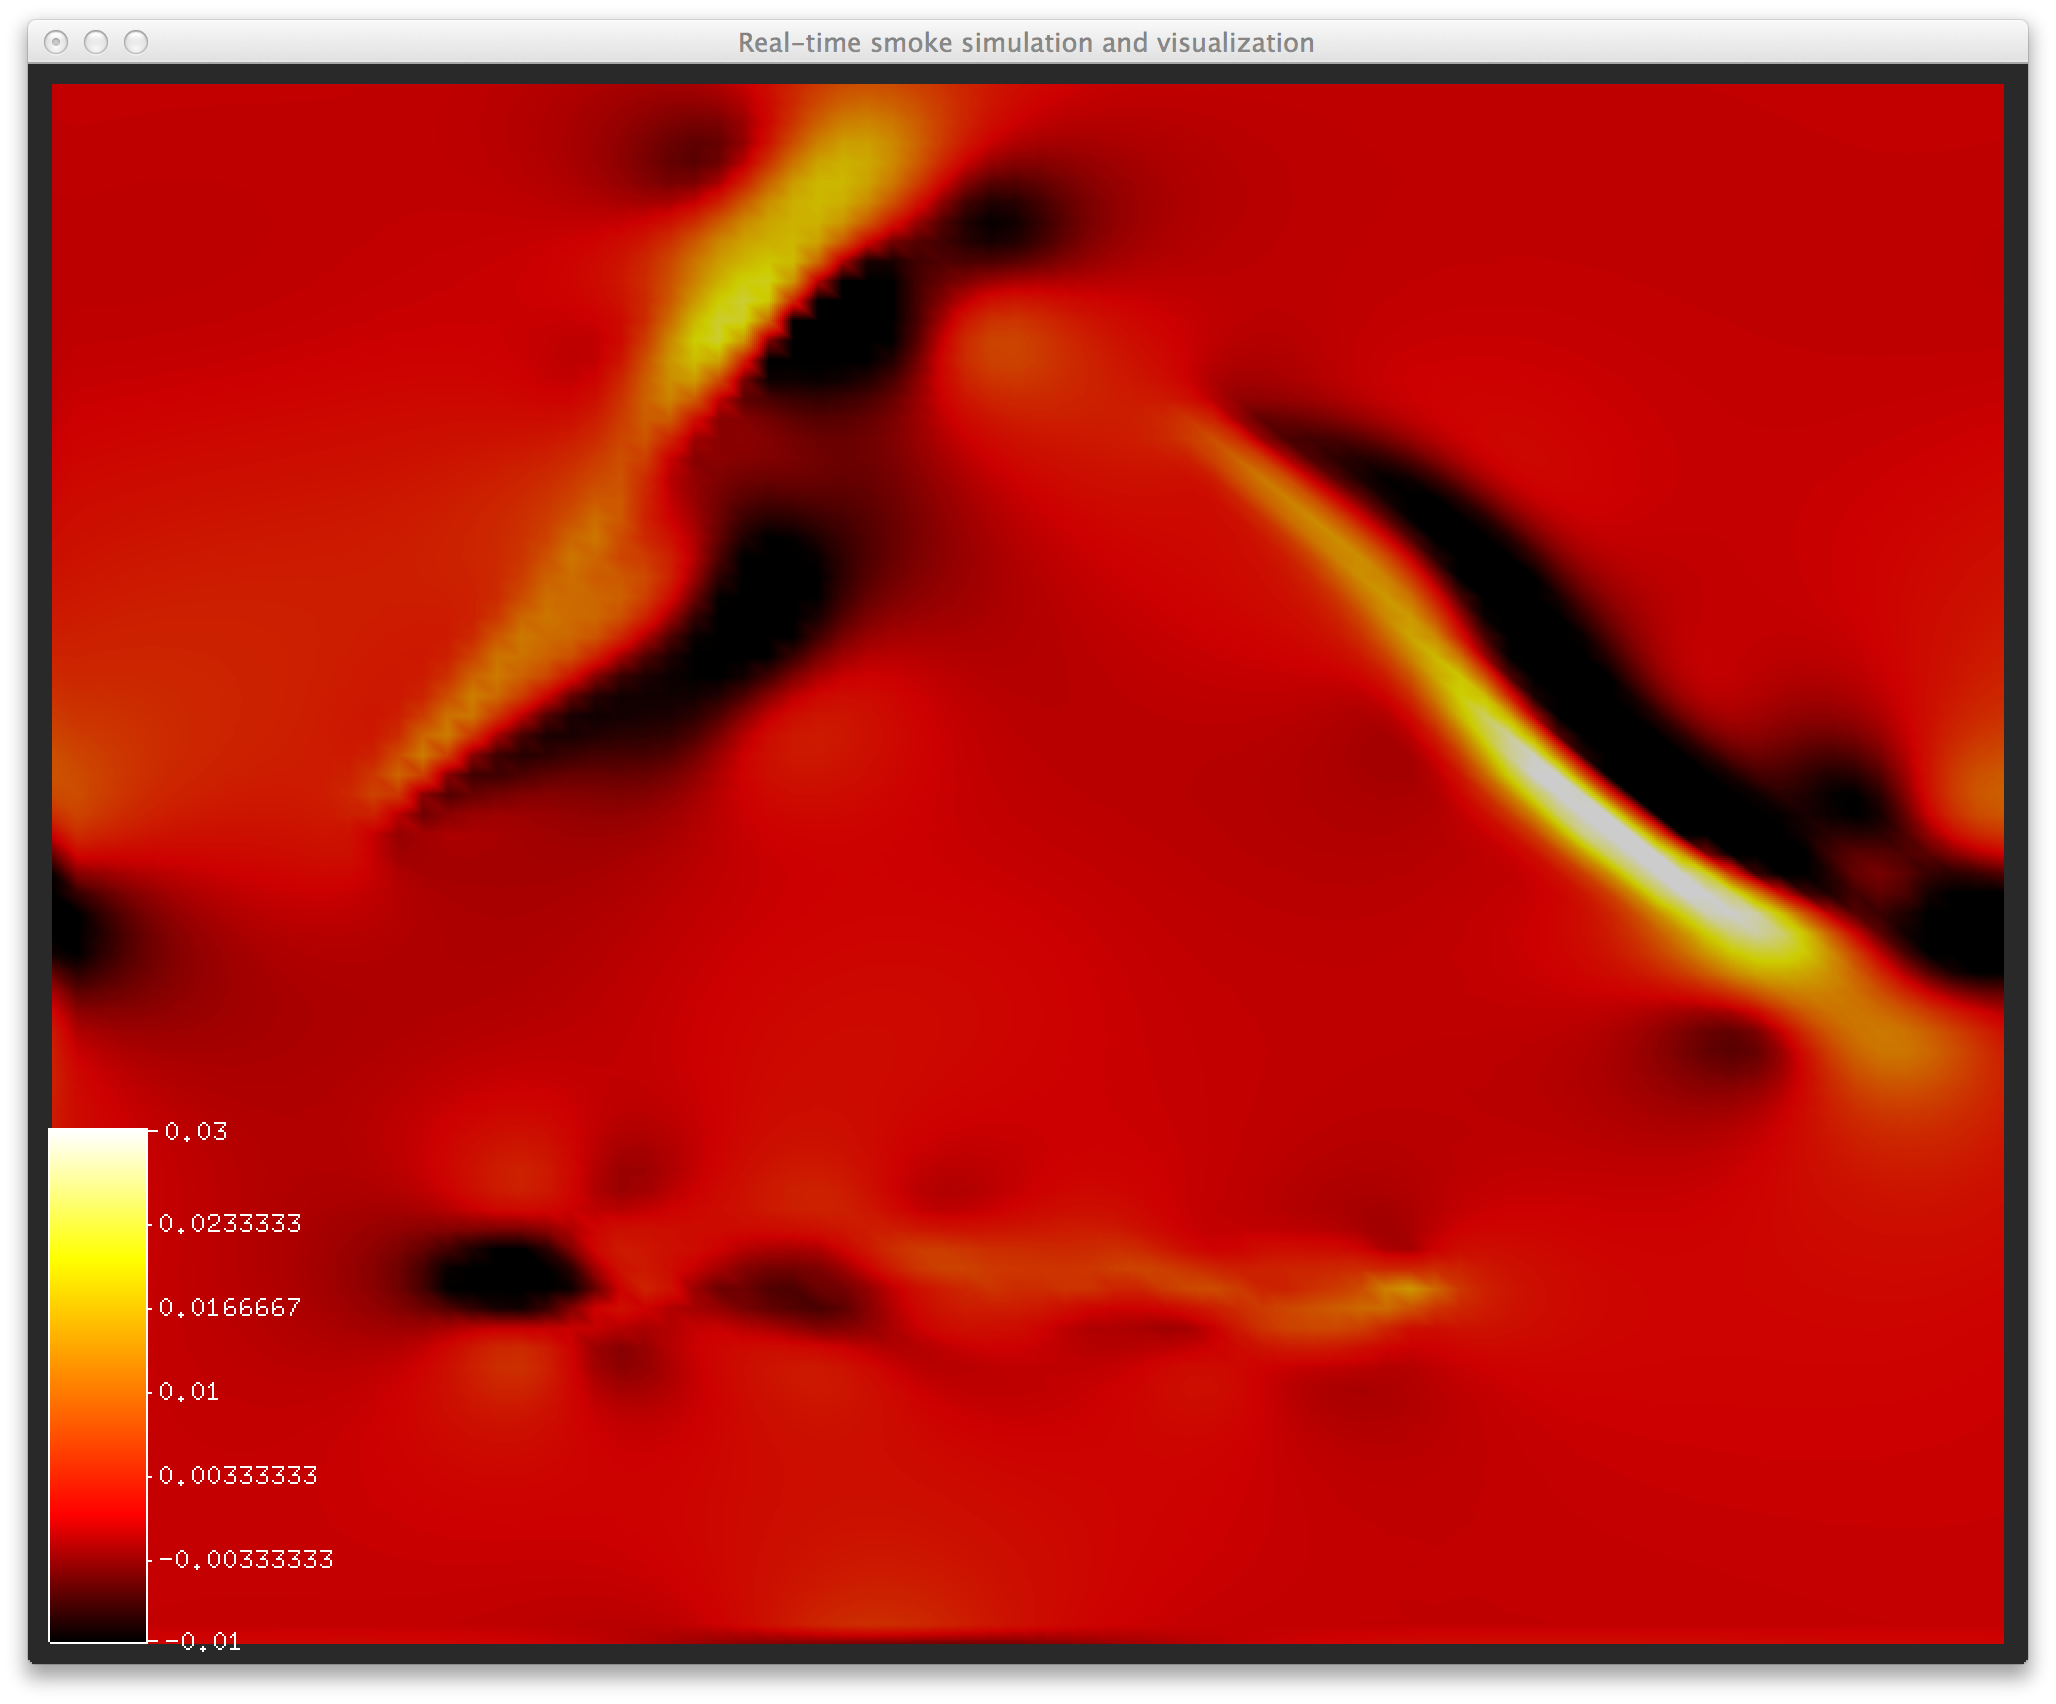
\includegraphics[height=3.5in]{figures/divergence/divergenceVelocity.png}
\caption{Velocity vector divergence on 80x80 regularly sampled grid coloured with a heatmap colormap.}
\label{fig:divergenceVelocity}
\end{center}
\end{figure}

Figure~\ref{fig:divergenceForce} illustrates ...

\begin{figure}[htbp]
\begin{center}
 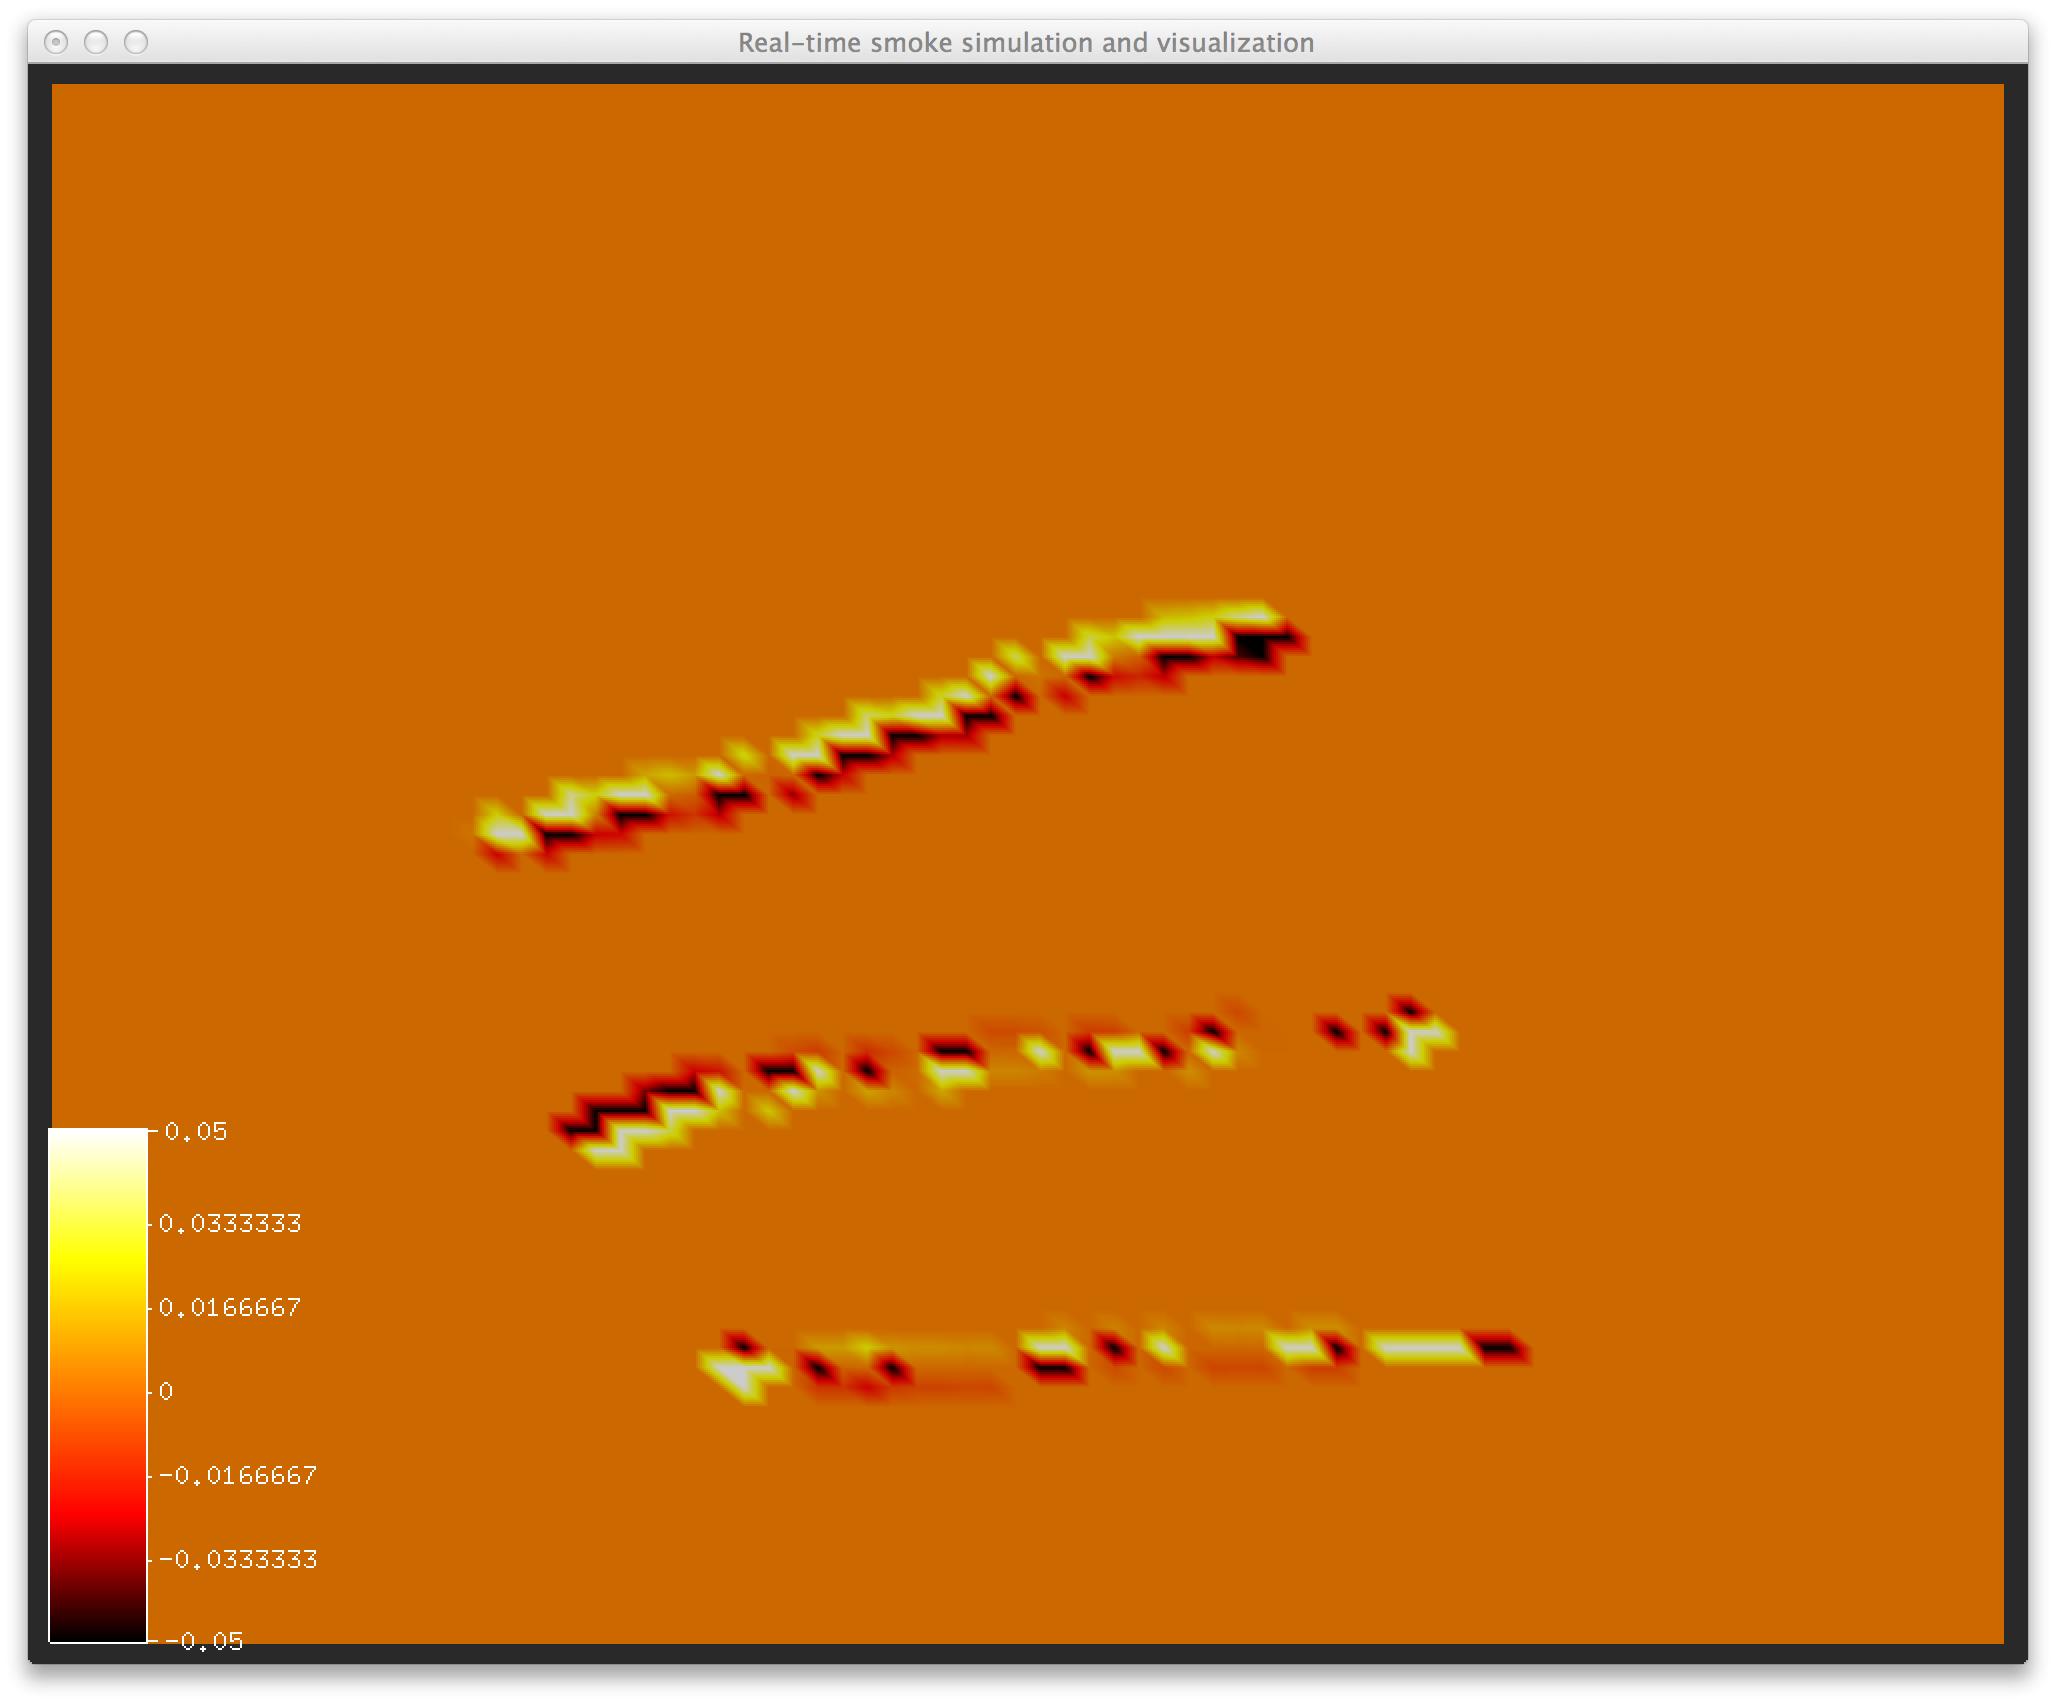
\includegraphics[height=3.5in]{figures/divergence/divergenceForce.png}
\caption{Force vector divergence on 80x80 regularly sampled grid coloured with a heatmap colormap.}
\label{fig:divergenceForce}
\end{center}
\end{figure}
